\mode*

\section{System model}%
\label{SystemModel}

\subsection{Assumptions}

We assume that every participant has a device similar to a smartphone.
(This means that we essentially provide a lower bound for the participation 
count, since some participants might not have any smartphone.)
It must be a portable device which can perform cryptographic operations and 
communicate with other devices during the protest, e.g.\ through an ad-hoc 
network.
I.e.\ no connection to the Internet is necessary during the protest.
During the protest these devices are computationally limited by their 
batteries.
Before and after the protest, we assume that the devices have Internet 
connections and are not computationally limited by any battery.

\mode<presentation>{%
\begin{frame}
  \begin{assumption}[During protest]
    \begin{itemize}
      \item Everyone has a smartphone.
      \item Can use ad-hoc networks during the event.
      \item Computations bounded by battery life.
    \end{itemize}
  \end{assumption}

  \pause{}

  \begin{assumption}[Before and after protest]
    \begin{itemize}
      \item Internet connection available.
      \item Computations not bounded by battery life.
    \end{itemize}
  \end{assumption}

  \pause{}

  \begin{remark}
    We provide a lower bound, since there might be participants without phones.
  \end{remark}
\end{frame}
}

We further assume that every participant has a digital certificate signed by 
some logically centralized certificate authority.
E.g.\ that we can use the cryptographic keys stored in the chip of the national 
identity card or passport.
We need this to prevent Sybil attacks~\cite{SybilAttack}.
\begin{frame}
\begin{remark}
  I.e.\ provided we can prevent Sybil.
\end{remark}
\end{frame}

\subsection{What is \protect\emph{a} protest?}%
\label{WhatIsAProtest}

Protests can vary considerably.
To be able to estimate the participation count for one, we first need to define
what should be counted.

Let us start by considering some examples.
During the demonstrations against the South Korean president in Seoul
\blockcquote{2016DemonstrationsInSeoul}{%
  \textins*{t}he rallies stretch\textins{ed} from midday to late night --- some 
  people stay\textins{ed} for several hours, others just several minutes%
}.
These rallies were all in the same location in the capital and repeated every 
weekend for the duration of a few weeks.
The Women's Marches~\cite{2017WomensMarchesInUS}, on the other hand, occurred 
in parallel in many locations.
We also have the Venezuelan demonstrations where
\blockcquote{2017VenezuelaProtestFrequency}{%
  anti-government demonstrators have staged daily protests across Venezuela%
} while
\blockcquote{AlJazeeraOnVenezuela2017}{%
  pro-government workers sang and danced as they staged a rival march to show 
  their support for the president's controversial plan to rewrite the 
  constitution%
}.
Judging from these examples, the minimal common part is the cause.

\mode<presentation>{%
\begin{frame}
  \begin{example}[Seoul 2016]
    \begin{itemize}
      \item Rallies every weekend.
      \item Starting midday, lasting to late night.
      \item Some stayed for several hours, some for only minutes.
    \end{itemize}
  \end{example}

  \pause{}

  \begin{example}[US 2017]
    \begin{itemize}
      \item Women's Marches in several locations.
      \item Marched some distance.
      \item One-time occurrence.
    \end{itemize}
  \end{example}
\end{frame}
}

\mode<presentation>{%
\begin{frame}
  \begin{example}[Venezuela 2017]
    \begin{itemize}
      \item Daily anti-government rallies.
      \item Multiple locations.
      \item Pro-government rallies too.
    \end{itemize}
  \end{example}
\end{frame}
}

The organizer Alice want to count everyone who participated at any time and in 
any of the locations~\cite{2016DemonstrationsInSeoul}.
(Whereas police are only interested in the maximum crowd at any point in time, 
to deploy enough personnel for crowd-control.)
We will define a protest as an event that is uniquely identified by its cause, 
its time and its location.
More specifically, we will use the following definition.

\begin{definition}[Protest]\label{DefProtest}
  A \emph{subprotest} is a tuple \((id; t_s, t_e; x, y)\), where
  \(id\in \Z_{2^\lambda}\) is an identifier,
  \((t_s, t_e)\in \R^2\) is a time interval,
  \((x, y)\in \R^2\) are the coordinates of the location.
  A \emph{protest} is a set of subprotests sharing the same \(id\).
\end{definition}

\mode<presentation>{%
\begin{frame}
\begin{definition}[Protest]
  \begin{itemize}
    \item A \emph{subprotest} is a tuple \((id; t_s, t_e; x, y)\), where
    \item \(id\in \Z_{2^\lambda}\) is an identifier,
    \item \((t_s, t_e)\in \R^2\) is a time interval,
    \item \((x, y)\in \R^2\) are the coordinates of the location.
    \item A \emph{protest} is a set of subprotests sharing the same \(id\).
  \end{itemize}
\end{definition}
\end{frame}
}

The protests described above can be captured using this definition by splitting 
them up into subprotests.
Each subprotest will then be captured by our definition and to find the total 
we can just sum up the results.

\begin{frame}
\begin{question}
  With this definition, can we participate in two sub-protests and be counted 
  twice?
\end{question}
\begin{remark}
  Perhaps not if linkability is tied to the cause.
\end{remark}
\end{frame}
\begin{remark}
  This sort of depends on the unique ring/list signature scheme that we use.
  As long as we can provide linkability between a user's proofs, we can consider 
  it the same protest.
  When we cannot, it must be a new protest.
  So this is supposedly decided by the one setting up the unique ring/list 
  signature scheme --- which we do not know yet how it will be done.
\end{remark}

Each participant who want to be counted must submit a participation proof.
The proof must be associated with the protest, i.e.\ contain its \(id\).
Furthermore it must provide the time and the location of the participation.
More formally, we define a participation proof as follows.

\begin{definition}[Participation proof]
  A \emph{participation proof} is a tuple \((id; t_s, t_e; lp; \sigma)\), where
  \(id, t_s, t_e\) are as in \cref{DefProtest},
  \(lp\) is a location proof and
  \(\sigma\) is a signature over the proof.
\end{definition}

\begin{frame}
  \mode<presentation>{%
  \begin{definition}[Participation proof]
    \begin{itemize}
      \item A \emph{participation proof} is a tuple \((id; t_s, t_e; lp; 
          \sigma)\), where
      \item \(id, t_s, t_e\) are as before,
      \item \(lp\) is a location proof and
      \item \(\sigma\) is a signature over the proof.
    \end{itemize}
  \end{definition}

  \pause{}
  }
\begin{question}
  How should this one relate to the \acp{LP} and blockchain?
\end{question}
\end{frame}

\begin{frame}
\begin{figure}
  \centering
  \begin{tikzpicture}
    \tikzset{grow'=right,level distance=5em}
    \Tree [.Proof
      [.{wsig} {\(x,y\)} [.{osig} [.{\(id\)} manifesto ] head ] [.tsig head'' ] ]
      {\dots}
      [.{wsig} {\dots} ]
    ]
  \end{tikzpicture}
  \mode<article>{%
    \caption{%
      The proof depends on several witness signatures (wsig), each of which 
      depends on the owner's signature (osig), which depends on the \(id\) of the
      protest and the head of the blockchain.
      Whenever possible, the witness signature should include proof that the 
      witness themself has been witnesses by a trusted witness (tsig).
    }
  }
\end{figure}
\end{frame}

\subsection{Adversary model}

We have three adversaries: Alice herself, Eve and Rusuk.
Alice the protest organizer tries to increase the count.
Eve the totalitarian dictator tries to decrease the count.
Additionally, Eve tries to deanonymize the participants.
Finally, we have Rusuk who is the head of another nation state.
Rusuk has some interest in affecting the state of Eve's regime, for Rusuk's own 
gain, thus supporting either Eve or Alice.
Rusuk will thus also try to either increase or decrease the count.

\mode<presentation>{%
\begin{frame}
  \begin{block}{Alice the activist}
    \begin{itemize}
      \item Alice organizes the protest against Eve's regime.
      \item Alice wants to have a high participation count.
      \item She tries to increase it.
    \end{itemize}
  \end{block}

  \pause{}

  \begin{block}{Eve the fake-news populist}
    \begin{itemize}
      \item Eve's regime is target of the protest.
      \item She wants to have a low participation count.
      \item She tries to decrease it.
    \end{itemize}
  \end{block}
\end{frame}
}

\mode<presentation>{%
\begin{frame}
  \begin{block}{Eve the totalitarian dictator}
    \begin{itemize}
      \item Eve wants to \enquote{convince} activists to support her.
      \item She wants to find all activists.
      \item She tries to identify (deanonymize) participants.
    \end{itemize}
  \end{block}
\end{frame}
}

\mode<presentation>{%
\begin{frame}
  \begin{block}{Rusuk the nation state}
    \begin{itemize}
      \item Rusuk benefits from the situation in Evestan.
      \item He wants the outcome to be the most beneficial.
      \item He will try to increase or decrease the participation count.
    \end{itemize}
  \end{block}
\end{frame}
}

More formally \dots


\mode<all>\endinput

\section{Old stuff}

We can divide the problem into three parts:
\begin{itemize}
  \item Register participants in the system.
  \item Collect the necessary data.
  \item Perform the counting and verification.
\end{itemize}

To register the participants we might be able to piggy-back on existing 
\acp{PKI} and blind signatures --- similarly as for voting systems.

There are several issues that must be treated:
\begin{itemize}
  \item Each location proof must be bound to one individual's participation.
    One protester must not be able to create two unique location proofs and be 
    able to increase the number of participants, that would violate 
    \cref{EligibilityVerif} above.
    In other words, we must prevent the Sybil attack.

  \item A group of people should not be able to generate \acp{LP} to make it 
    look as if they participated in the protest but actually stayed at home.
    This means that all \acp{LP} must be linked to each other.
    If a protest has hundreds of thousands of participants, then this linking 
    must be achieved efficiently.
\end{itemize}

The model will be a public anonymous blackboard.
We will use this blackboard to publish locations proofs after the protest.

We want the following properties:
\begin{description}
  \item[Correctness] We want to count everyone once and only once.
  \item[Unforgeability] Participation should not be possible to forge.
    I.e.\ non-participants should not be able to say they were present.
    This together with correctness will provide authenticity to the protest 
    verification.
  \item[Anonymity] Given the data published on the blackboard, the adversary 
    should not be able to tell two participants apart.
  \item[Decentralized] There should be no central authority.
\end{description}

Can the adversary publish a public-key looking random string to sabotage the 
blackboard?

Basically the properties that we are interested in are similar to those of 
electronic voting, so we would like to reuse as many definitions from there as 
possible.

\subsection{Decentralization}

In \ac{PROPS} the prover must have a secret signed by \iac{CA}.
This \ac{CA} can be implemented as a secret-sharing scheme.
Usually these have a fixed threshold \((t, n)\).
This can be achieved by commitments, then the shared secret is computed.
However, it would be interesting to have the threshold dynamically adapt to the 
number of participants, i.e.\ participants can join later too.

Can the adversary then \enquote{join} enough many to throw off the threshold?

\subsection{Correctness and Unforgeability}

Each prover must reach a threshold of witnesses \(k\).
We must be able to prevent a prover to collect \(2k\) witnesses and then 
publishing two proofs.
We therefore must achieve conditional linkability between the \acp{LP} 
published on the blackboard.
If a second \ac{LP} for a secret is published, then those should be linkable.
This might be possible to achieve with unique group 
signatures~\cite{UniqueGroupSignatures,UniqueRingSignatures,ListSignatures}.


